Clase: 20/09/2022

\begin{teorema}[Fundamental del álgebra (Gauss)]
    Sean $a_0,a_1,\cdots, a_n$, números complejos $n\geq 1,a_n\neq 0$. Si $p(x)=a_0+a_1z+a_2z^2+\cdots + a_nz^n$, entonces existe $z_0\in\mathbb{C}\ni p(z_0)=0$
    \begin{dem}
        Suponga, por el absurdo que $p(z)\neq 0,\forall z\in \mathbb{C}$. Sea $f(z)=\frac{1}{p(z)}$. Como $p(z)\neq 0\implies f(z)$ es entera (cociente de funciones analíticas), y además, como $a_n\neq 0,f(z)$ no es constante. A probar: $f$ es acotada $\forall z\in \mathbb{C}\implies$ Por Liouville, $f$ es constante $(\to\gets)$. 
    \end{dem} 
\end{teorema}

\begin{lema}
    Sea $f$ una función continua sobre la región $G\subseteq \mathbb{C}$. Sean $z_1,z_2\in G$ y $\gamma_0$ y $\gamma_1$, curvas que unen a $z_1$ y $z_2$ en $G\ni ¿$
    $$\int_{\gamma_0}f=\int_{\gamma_1}f$$
    Entonces, existe una función analítica $F\ni F'(z)=f(z),\forall z\in G$. 
    \begin{figure}[H]
        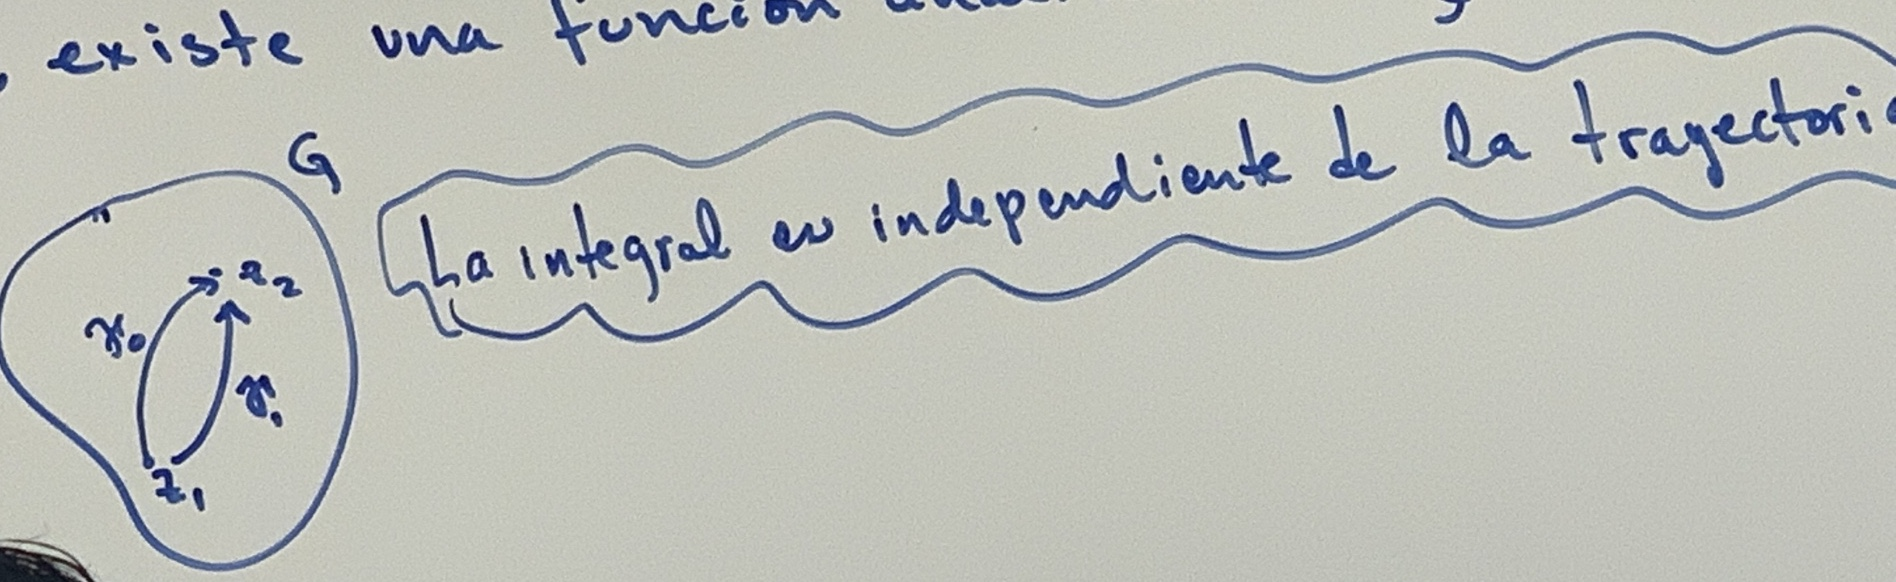
\includegraphics[scale=0.2]{imagenes/15.jpeg}
    \end{figure}
    \begin{dem}
        \begin{figure}[H]
            \centering
            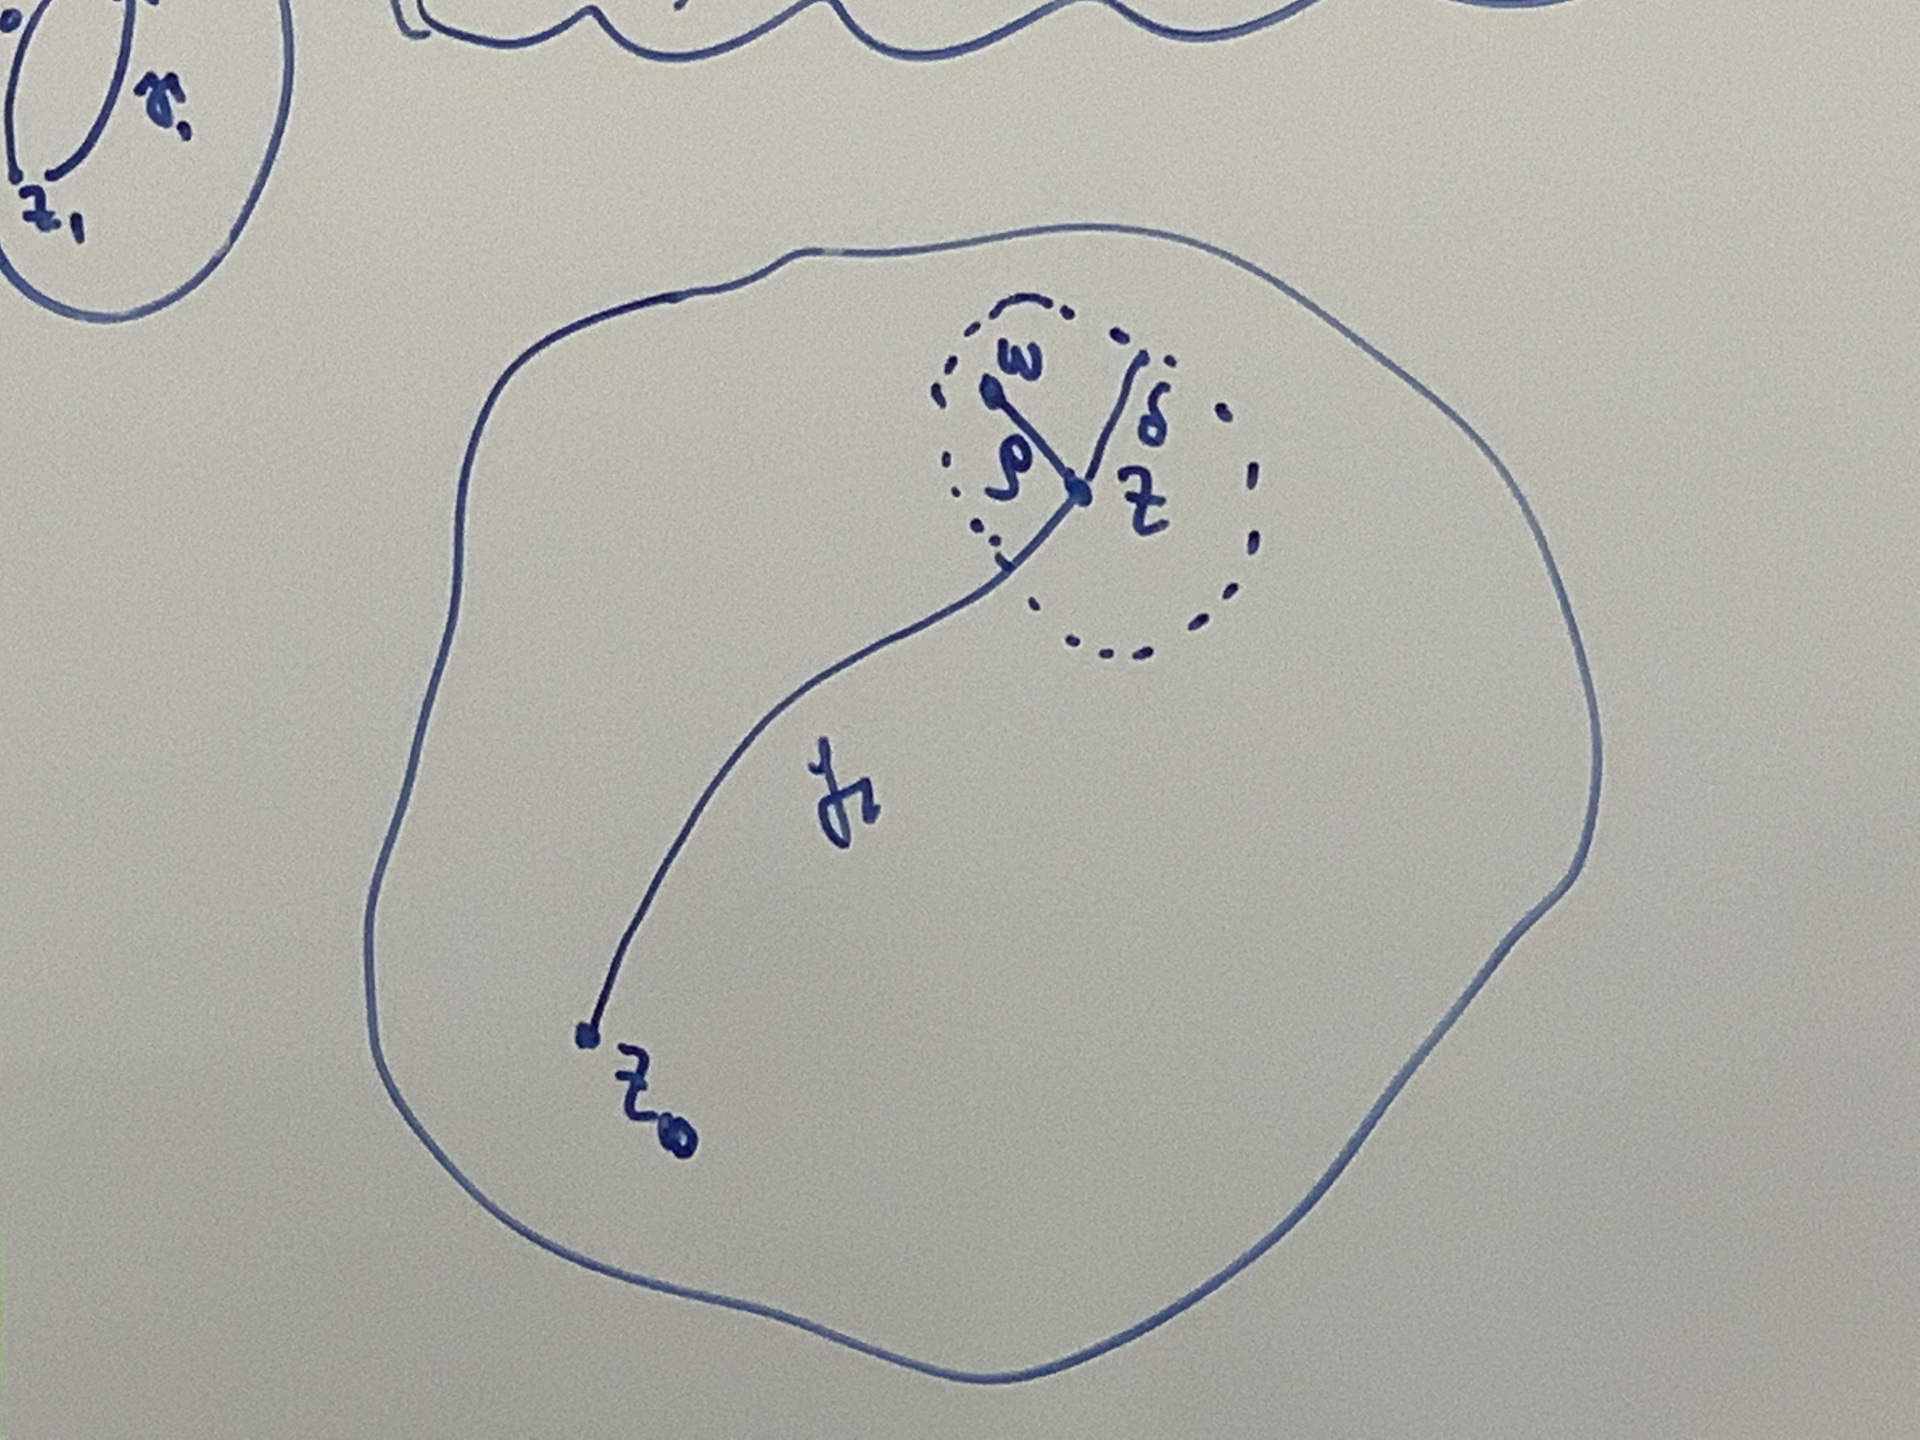
\includegraphics[scale=0.1]{imagenes/15.1.jpeg}
        \end{figure}
            Sea $F(z)=\int_{z_0}^zf(\psi)d\psi$, tal que 
            \begin{itemize}
                \item Como $f$ es continua en $G\implies f$ es continua en $z\in G\implies \forall \varepsilon>0\exists \delta>0\ni |w-z|<\delta \implies  |f(w)-f(z)|<\varepsilon$
                \item Sea $w\in D(z,\delta)$, y sea $\rho$ la recta que une $w$ con $z$. \begin{align*}
                    \left|\frac{F(w)-F(z)}{w-z}-f(z)\right| &=\left| \frac{F(w)-F(z)-f(z)(w-z)}{w-z}\right|\\
                    &= \left|\frac{\int_{\gamma+\rho}f - \int_\gamma f - f(z)\int_\rho 1\cdot d\psi}{w-z}\right|\\
                    &= \left| \frac{\int_\rho f- f(z)\int_\rho 1d\psi}{w-z}\right|\\
                    &= \frac{1}{|w-z|} \left| \int_\rho[f(\psi)-f(z)]d\psi\right|\\
                    &<\frac{1}{|w-z|}\in |w-z|\\
                    &< \varepsilon
                \end{align*}
            \end{itemize}
        
    \end{dem}
\end{lema}

\begin{teorema}[Morera]
    Sea $f$ una función continua sobre una región $G\subseteq \mathbb{C}$, y suponga que $\int_\gamma f=0$, para cualquier curva cerrada $\gamma$ sobre $G$. Entonces, $f$ es analítica sobre $G$ y se tiene que $f=F'$, para alguna función analítica $F$ sobre $G$.  
\end{teorema}
\begin{cajita}
    \begin{teorema}[Cauchy-recordatorio]
        Si $f$ es analítica sobre $y$ en el interior de una curva cerrada $\gamma$, entonces 
        $$\int_\gamma f=0$$ 
    \end{teorema}
\end{cajita}
\begin{dem}
    Como $f$ es continua sobre $G$ y la integral es independiente de la trayectoria $\implies \exists F$, función analítica sobre $G$, tal que $F'=f\implies F'' = f'\implies f$ es analítica sobre $G$. 
\end{dem}


\subsection{Series}

\begin{definicion}
    Una serie de números complejos $\sum_{k=1}^{\infty}a_k$ converge a $S$, denotado $\sum a_k=S$, si la sucesión $S_n=\sum_{k=1}^n a_k$ converge a $S$. 
\end{definicion}

\begin{definicion}
    La sucesión $(z_n)\subseteq \mathbb{C}$ es de Cauchy si y solo si $\forall \varepsilon>0\exists N\in\mathbb{Z}^+\ni$ si $n,m\geq N\implies |z_n-z_m|<\varepsilon$. 
\end{definicion}

\begin{teorema}
    Tenemos, 
    \begin{enumerate}
        \item Si $\lim a_n$ existe $\implies $ es única. 
        \item Una sucesión $(z_n)$ es convergente si y solo si $(z_n)$ es de Cauchy. 
    \end{enumerate}
\end{teorema}


\begin{nota}
    \begin{enumerate}
        \item $(z_n)$ es de Cauchy, si $\forall \varepsilon >0\exists N\in\mathbb{Z}^+\ni |z_n-z_{m+p}|<\varepsilon,\forall n\geq N,\forall p=1,2,3,\cdots
        $
        \item $\sum_{k=1}^\infty a_k$ converge (si y solo si)* $\forall \varepsilon>0\exists N\in \mathbb{Z}^+\ni n\geq N\implies |\sum_{k=n+1}^{n+p}a_k|<\varepsilon, \forall p=1,2,\cdots$
        \item En (2) hagamos $p=1$. $\implies$ si $\sum_{k=1}^{\infty}a_k$ converge $\implies |a_n|\to 0$
        \item Nótese que $\sum_{k=1}^\infty 1/k$ es tal que la serie diverge aunque $|1/k|\to 0$. (El converso de (3) no se cumple).
    \end{enumerate}
    
\end{nota}

\begin{definicion}
    Una serie en los complejos $\sum a_k$ converge absolutamente, si $\sum |a_k|$ converge. 
\end{definicion}

\begin{teorema}
    Si $\sum a_k$ sobre $\mathbb{C}$ es absolutamente convergente $\implies \sum a_k$ converge. 
     
\end{teorema}